\begin{refsection}

\chapter{Variants of folate metabolism genes and the risk of non-syndromic CTHD} % Main chapter title
\chaptermark{Variants of folate metabolism genes}

\label{Chapter6} % Change X to a consecutive number; for referencing this chapter elsewhere, use \ref{ChapterX}

%----------------------------------------------------------------------------------------
%	SECTION 1
%----------------------------------------------------------------------------------------

\section{Introduction}

Prevention of CTHD has been hampered by a lack of information about modifiable risk factors for abnormalities in cardiac development. Despite this, clinical research and epidemiological data suggests that maternal preconception folic acid supplementation would reduce the occurrence of CTHD by 40–60\% \cite{smedts2008maternal,rosenquist1996homocysteine,botto2003multivitamin,boot2004cardiac}. Further evidence is reflected in the fact the folate antagonists increase the risk of CHD \cite{bailey2005folic}. 

Folate acts as a one-carbon donor, which is involved in both the de novo synthesis of nucleotides and methyl transfer reactions. A number of polymorphisms in folate pathway genes have been identified that appear to affect protein function and/or folate metabolism and thus may affect the risk for heart defects \cite{bailey2009folate}. Therefore exploring the association between genetic variants in genes involved in folate metabolism pathway and the risk of CTHD will possibly shed light on the mechanism how folate carries out its protection effects. On this basis, for this study six variants were chosen to test for an association between genotype and disease: rs1801133, rs1801131 of methylenetetrahydrofolate reductase (\textit{MTHFR}), rs1051266 of solute carrier family 19 (\textit{SLC19A1}), rs1805087 of methionine synthase (\textit{MTR}) and rs1801394 and rs1532268 of methionine synthase reductase (\textit{MTRR}). These polymorphisms were selected on the basis of their reported associations with risk for neural tube defects, and observations of cardiac defects in mouse models.

\begin{sloppypar}\textit{MTHFR} plays a central role in folate metabolism where it irreversibly converts 5, 10-methylenetetrahydrofolate to 5-methylenetetrahydrofolate, the primary circulating form of folate. It is believed that the rs1801133 variant (TT) decreases \textit{MTHFR} activity and increases the homocysteine level. Similarly the rs1801131variant (CC) also reduces enzyme activity but to a lesser degree than the rs1801133 variant. Another key gene \textit{MTR} catalyzes the remethylation of homocysteine to methionine, required for production of S- adenosylmethionine, the universal methyl group donor. The A to G polymorphism at position 2756 in the protein binding region of \textit{MTR} replaces aspartic acid with glycine and it has been suggested that plasma homocysteine level is lower in those with the rarer, G, than the more common, A, allele. \textit{MTR} is maintained in its active form by \textit{MTRR}. The A66G SNP in the \textit{MTRR} gene results in the substitution of isoleucine with methionine and another SNP C524T leads to an amino acid change from serine to leucine. Subjects homozygous for the common allele have elevated homocysteine levels compared with those who had other genotypes. \textit{SLC19A1} is involved in the transport of folate and the regulation of intracellular concentrations of folate. This SNP is an A-to-G change replacing a histidine with an arginine in the protein. Higher plasma folate levels were observed in normal homozygotes(AA) individuals when compared with  the homozygote variant (GG) individuals \cite{bailey2009folate}.\end{sloppypar}

Thus, as demonstrated by the functional role of these genes, investigating possible gene-gene and gene-environment interactions in the etiology of CTHD is a prudent research approach owing to what is currently recognized about these defects. Moreover, confirmation of an association between CTHD and the folate metabolic pathway would suggest potential, targeted risk reduction strategies. 

\section{Methodology}

DNA was isolated from the peripheral blood of 96 cases and 100 controls as detailed in section 2.3.3. The quality and quantity was confirmed by agarose gel electrophoresis and nanodrop estimation respectively. The isolated DNA was amplified with appropriate primers as described in \cref{tab:6_1}. Briefly, 50 ng of DNA was amplified with 62.5 ng/ µl of each specific primer in a final volume of 20 µl. Direct dye terminator sequencing of PCR products was performed using the ABI Prism Big Dye Terminator V.1.1 according to the manufacturer’s instructions (ABI, Foster City, CA, USA). SNP genotyping was conducted using an ABI 3730 automated sequencer and analyzed using SeqScape analysis software V2.5.

\begin{landscape}
\begin{table}[!tb]
\centering
\caption{PCR primers and reaction conditions used to amplify the selected genes of folate metabolism \cite{deeparani2009detection,shaw2003genetic,galbiatti20105,zeng2011a66g}}
\label{tab:6_1}
\begin{tabular}{  l P{1in} P{0.75in} p{4.3in}  }
\toprule
	\textbf{Polymorphism} & \textbf{Amplicon Size (bp)} & \textbf{Tm (ºC)} & \textbf{Primer sequence} \\ \toprule
	\textit{MTHFR}: rs1801133 C>T & 198 & 65 & F: 5’TGAAGGAGAAGG TGTCTGCGGGA 3’ \\ 
	 &  &  & R: 5’AGGACGGTGCG TGAGAGTG 3’ \\ \midrule
	\textit{MTHFR}: rs1801131 A>C & 128 & 65 & F: 5' CAAGGAGGAGCT  GCTGAAGA 3’ \\ 
	 &  &  & R: 5' CCACTCCAGCAT CACTCACT 3’ \\ \midrule
	\textit{SLC19A1}:  rs1051266  G>A & 140 & 56 & F: 5' AG TGT CAC CTT CGT CCC 3' \\ 
	 &  &  & R: 5' TCC CGC GTG AAG TTC TTG 3' \\ \midrule
	\textit{MTR}: rs1805087A>G & 498 & 56 & F: 5’CCA GGG TGC GAC GTA TAC AG 3’ \\ 
	 &  &  & R: 5’GCC TTT TAC ACT CCT CAA AACC 3’. \\ \midrule
	\textit{MTRR}:  rs1801394 A>G & 151 & 65 & F: 5'CAAAGGCCATCGCAGAAGACAT3' \\ 
	 &  &  & R:5'AAACGGTAAACGGTAAAATCCACTGTAACGGC3' \\ \midrule
	\textit{MTRR}:  rs1532268 C>T & 300 & 59 & F:5' GTCAAGCAGAGGACAAGAG 3' \\ 
	 &  &  & R:5' AGAGACTCCTGCAGATGTAC 3' \\ \bottomrule
\end{tabular}
\end{table}
\end{landscape}

\section{Statistical Analysis}

Differences in the allele and genotype frequency of the six SNPs observed between the cases and controls were evaluated using the Student's t test (for continuous variables) and χ$^2$ test (for categorical variables). The associations between the six SNP and risk of CTHDs were estimated by calculating the odds ratios (OR) and their 95\% confidence intervals (CIs) from logistic regression analyses. All of the statistical analyses were performed with Statistical Package for Social Sciences (SPSS) software (version 19.0). 

An interaction analysis using the multifactor dimensionality reduction (MDR) method was also performed to investigate whether specific combinations of genotypes across all six loci contributed to the disease status. Finally, the potential association between the risk genotypes and maternal multivitamin intake was also assessed using Pearsons Chi square analysis. 

\section{Results}
\subsection{Hardy–Weinberg Equilibrium}

\begin{sloppypar}The primary information for the six genotyped SNPs is shown in \cref{tab:6_2}. The observed genotype frequencies for \textit{MTHFR}: rs1801131 A>C and \textit{MTR}: rs1805087A>G were in Hardy–Weinberg equilibrium (HWE) in both the cases and controls. However, the remaining four polymorphisms showed a departure from HWE. \cref{fig:6_1,fig:6_2,fig:6_3} show the genotypes observed for each of the studied genes.\end{sloppypar}

\begin{table}[!tb]
\centering
\caption{Primary information for six genotyped SNPs}
\label{tab:6_2}
\begin{tabular}{ l P{0.75in} P{0.75in} P{0.75in} P{0.75in} }
\toprule
	\textbf{Genotyped SNPs} & \textbf{Global MAF} & \textbf{MAF in study controls} & \textbf{P-value for study cases} & \textbf{P-value for study controls}   \\ \toprule
	 
	\textit{MTHFR}: rs1801133 C>T & 0.32 & 0.09 & 0.96 & 0.35  \\ \midrule
	\textit{MTHFR}: rs1801131 A>C & 0.22 & 0.32 & <0.05 & <0.05  \\ \midrule
	\textit{SLC19A1}: rs1051266  G>A & 0.49 & 0.37 & <0.05 & <0.05  \\ \midrule
	\textit{MTR}: rs1805087A>G & 0.19 & 0.35 & 0.07 & 0.39  \\ \midrule
	\textit{MTRR}: rs1801394 A>G  & 0.37 & 0.44 & <0.05 & <0.05  \\ \midrule
	\textit{MTRR}: rs1532268 C>T & 0.25 & 0.26 & <0.05 & <0.05  \\ \bottomrule
\multicolumn{5}{l}{\textsuperscript{*}\footnotesize{MAF: minor allele frequency, obtained from www.ncbi.nlm.nih.gov/snp}}\\
\end{tabular}
\end{table}





\begin{table}[!tb]
\centering
\caption{Distribution of \textit{MTHFR}: rs1801133 C>T genotype and allele frequencies}
\label{tab:6_3}
\begin{tabular}{  P{1.25in} P{0.5in} P{0.5in} P{0.5in} P{0.5in} P{0.5in} P{0.5in} }
\toprule
	\multirow{2}{*}{\textbf{Subjects}} & \multicolumn{3}{c}{\textbf{Genotype Frequency}} &  \multicolumn{2}{c}{\textbf{Allele Frequency}} &  \textbf{P} \\ 
	
	 & CC & CT & TT & C & T &  \\ \toprule
	Cases (n=96) & 95 & 1 & 0 & 0.99 & 0.01 & NS \\ \midrule
	Controls(n=100) & 83 & 17 & 0 & 0.91 & 0.09 & NS \\ \bottomrule
\multicolumn{7}{l}{\textsuperscript{*}\footnotesize{NS: not significant}}\\
\end{tabular}
\end{table}

\begin{table}[!tb]
\centering
\caption{Distribution of \textit{MTHFR}: rs1801131 A>C genotype and allele frequencies}
\label{tab:6_4}
\begin{tabular}{  P{1.25in} P{0.5in} P{0.5in} P{0.5in} P{0.5in} P{0.5in} P{0.5in} }
\toprule
	\multirow{2}{*}{\textbf{Subjects}} & \multicolumn{3}{c}{\textbf{Genotype Frequency}} &  \multicolumn{2}{c}{\textbf{Allele Frequency}} &  \textbf{P} \\
	
	 & AA & AC & CC & A & C &  \\ \toprule
	Cases (n=96) & 27 & 32 & 37 & 0.32 & 0.68 & <0.05 \\ \midrule
	Controls (n=100) & 58 & 20 & 22 & 0.55 & 0.45 & <0.05 \\ \bottomrule
\end{tabular}
\end{table}

\begin{table}[!tb]
\centering
\caption{Distribution of \textit{SLC19A1}: rs1051266 G>A genotype and allele frequencies}
\label{tab:6_5}
\begin{tabular}{  P{1.25in} P{0.5in} P{0.5in} P{0.5in} P{0.5in} P{0.5in} P{0.5in} }
\toprule
	\multirow{2}{*}{\textbf{Subjects}} & \multicolumn{3}{c}{\textbf{Genotype Frequency}} &  \multicolumn{2}{c}{\textbf{Allele Frequency}} &  \textbf{P} \\
	& GG & GA & AA & G & A &  \\ \toprule
	Cases (n=96) & 39 & 30 & 27 & 0.56 & 0.44 & <0.05 \\ \midrule
	Controls (n=100) & 48 & 30 & 22 & 0.63 & 0.37 & <0.05 \\ \bottomrule
\end{tabular}
\end{table}

\begin{table}[!tb]
\centering
\caption{Distribution of \textit{MTR}: rs1805087 A>G genotype and allele frequencies}
\label{tab:6_6}
\begin{tabular}{  P{1.25in} P{0.5in} P{0.5in} P{0.5in} P{0.5in} P{0.5in} P{0.5in} }
\toprule
	\multirow{2}{*}{\textbf{Subjects}} & \multicolumn{3}{c}{\textbf{Genotype Frequency}} &  \multicolumn{2}{c}{\textbf{Allele Frequency}} &  \textbf{P} \\
	& AA & AG & GG & A & G &  \\ \toprule
	Cases n=96) & 41 & 37 & 18 & 0.65 & 0.35 & NS \\ \midrule
	Controls (n=100) & 41 & 49 & 10 & 0.62 & 0.38 & NS \\ \bottomrule
\end{tabular}
\end{table}	

\begin{table}[!tb]
\centering
\caption{Distribution of \textit{MTRR}: rs1801394 A>G genotype and allele frequencies}
\label{tab:6_7}
\begin{tabular}{  P{1.25in} P{0.5in} P{0.5in} P{0.5in} P{0.5in} P{0.5in} P{0.5in} }
\toprule
	\multirow{2}{*}{\textbf{Subjects}} & \multicolumn{3}{c}{\textbf{Genotype Frequency}} &  \multicolumn{2}{c}{\textbf{Allele Frequency}} &  \textbf{P} \\
	& AA & AG & GG & A & G &  \\ \toprule
	Cases (n=96) & 9 & 68 & 15 & 0.44 & 0.56 & <0.05 \\ \midrule
	Controls (n=100) & 2 & 83 & 15 & 0.45 & 0.55 & <0.05 \\ \bottomrule
\end{tabular}
\end{table}

\begin{table}[!tb]
\centering
\caption{Distribution of \textit{MTRR}: rs1532268 C>T genotype and allele frequencies}
\label{tab:6_8}
\begin{tabular}{  P{1.25in} P{0.5in} P{0.5in} P{0.5in} P{0.5in} P{0.5in} P{0.5in} }
\hline
	\multirow{2}{*}{\textbf{Subjects}} & \multicolumn{3}{c}{\textbf{Genotype Frequency}} &  \multicolumn{2}{c}{\textbf{Allele Frequency}} &  \textbf{P} \\
	& CC & CT & TT & C & T &  \\ \toprule
	Cases (n=96) & 0 & 44 & 52 & 0.26 & 0.74 & <0.05 \\ \midrule
	Controls (n=100) & 0 & 51 & 49 & 0.23 & 0.27 & <0.05 \\ \bottomrule
\end{tabular}
\end{table}

\begin{sidewaysfigure}[hp]
\centering
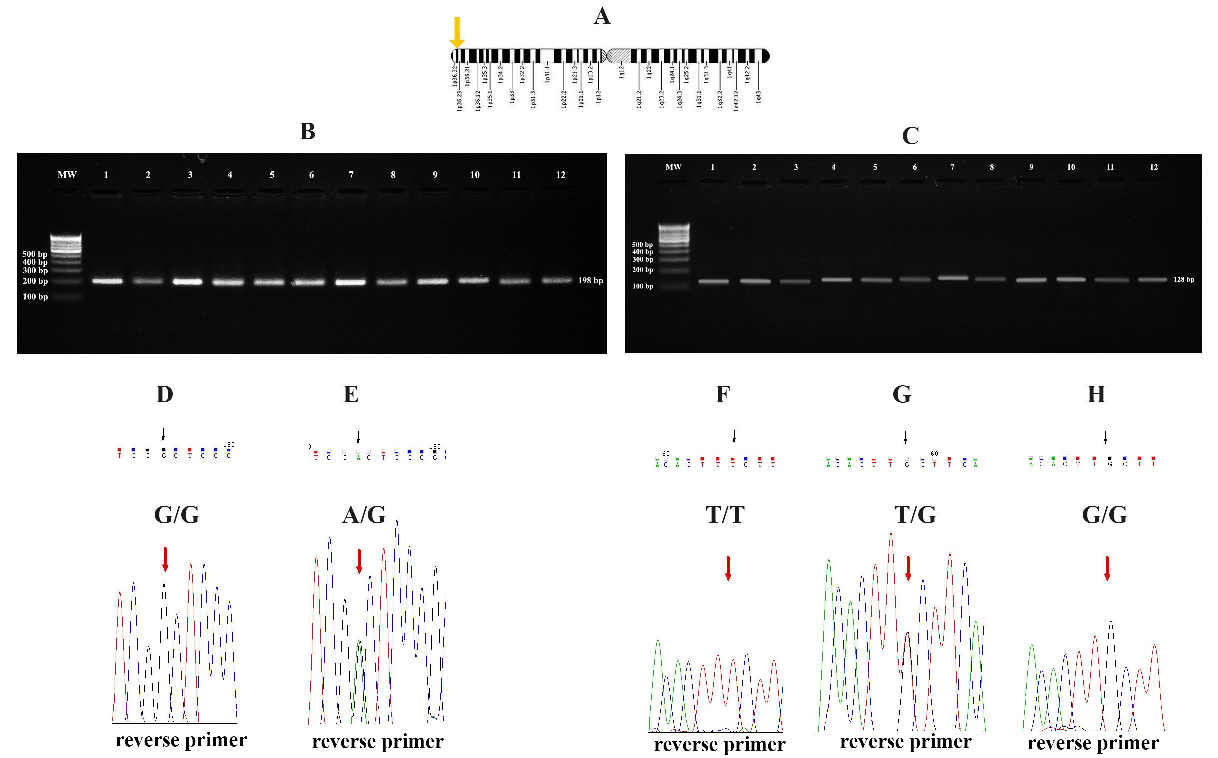
\includegraphics[scale=0.9,keepaspectratio]{Figures/Figure6_1.pdf}
\rule{35em}{0.5pt}
\caption{\textbf{SNP observed in the \textit{MTHFR} gene}
\textbf{A.} Schematic representation of the \textit{MTHFR} gene. \textbf{B, C.} 2\% agarose gel image showing the representative amplicons of \textit{MTHFR}: rs1801133 C>T (198bp) and \textit{MTHFR}: rs1801133 C>T (128 bp) respectively \textbf{D-H.} Sequence chromatogram showing the genotypes detected, with the arrows indicating the G/G and A/G genotypes (using the reverse primer) of \textit{MTHFR}: rs1801133 C>T and T/T, T/G and G/G genotypes of \textit{MTHFR}: rs1801133 C>T (using the reverse primer) respectively}
\label{fig:6_1}
\end{sidewaysfigure}

\begin{sidewaysfigure}[hp]
\centering
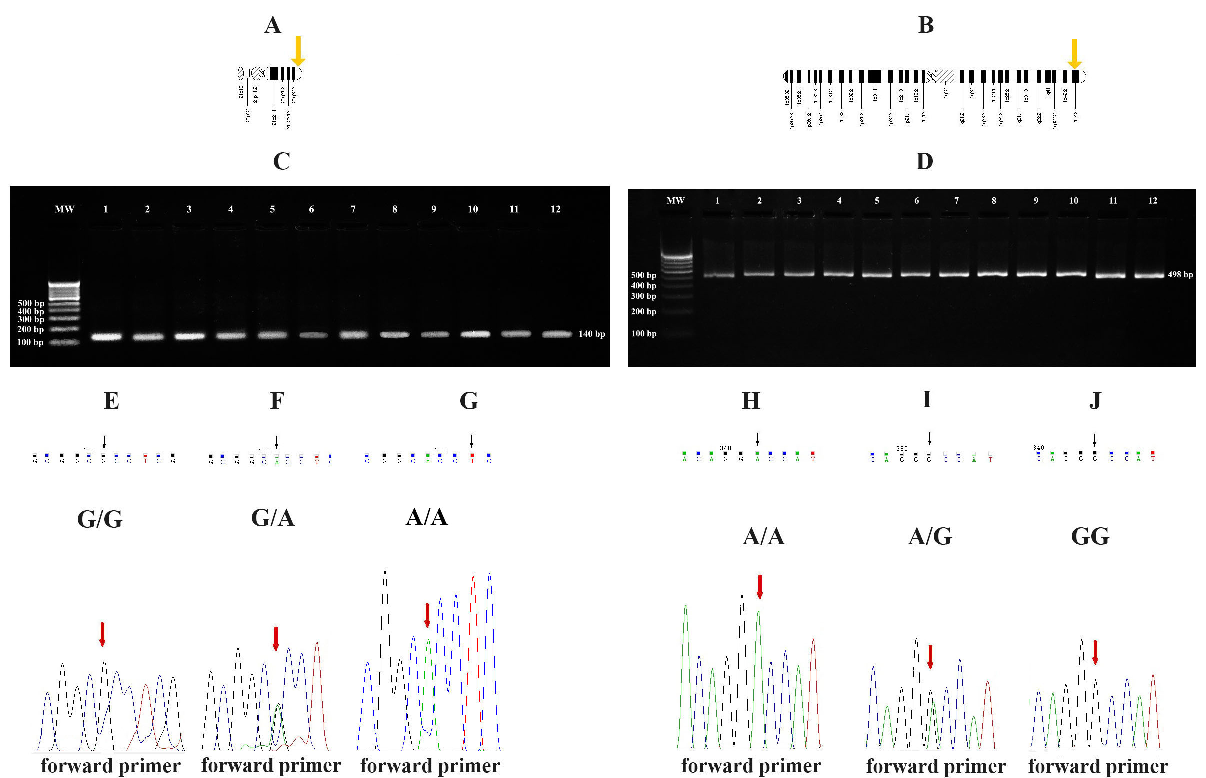
\includegraphics[scale=0.9,keepaspectratio]{Figures/Figure6_2.pdf}
\rule{35em}{0.5pt}
\caption{\textbf{SNP observed in the \textit{SLC19A1} and \textit{MTR} genes}
\textbf{A.} Schematic representation of the \textit{SLC19A1} and \textit{MTR} gene. \textbf{B, C.} 2\% agarose gel image showing the representative amplicons of \textit{SLC19A1}:  rs1051266 G>A (140 bp) and \textit{MTR}: rs1805087A>G (498 bp) respectively \textbf{D-J.} Sequence chromatogram showing the genotypes detected with the arrows indicating the G/G, G/ and TT (using the forward primer) genotypes of \textit{SLC19A1}:  rs1051266  and A/A, A/G and G/G genotypes of \textit{MTR}: rs1805087A>G (using the forward primer) respectively}
\label{fig:6_2}
\end{sidewaysfigure}

\begin{sidewaysfigure}[hp]
\centering
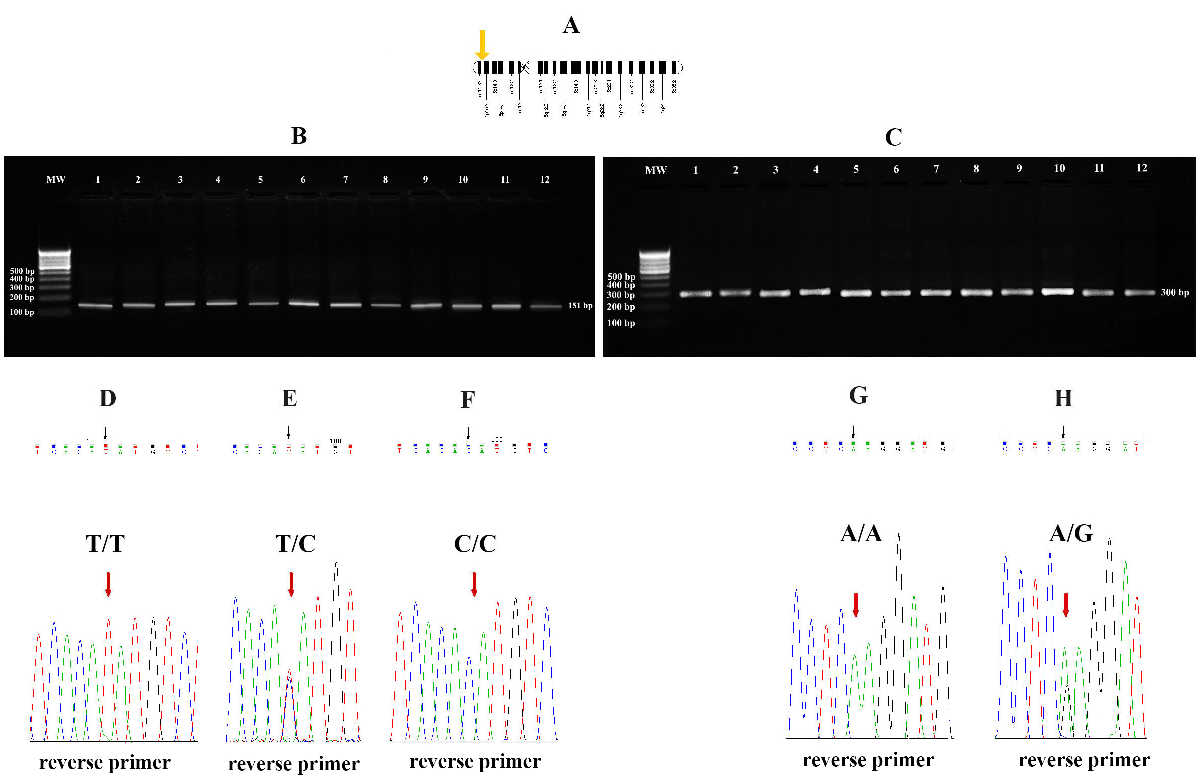
\includegraphics[scale=0.9,keepaspectratio]{Figures/Figure6_3.pdf}
\rule{35em}{0.5pt}
\caption{\textbf{SNP observed in the \textit{MTRR} gene}
\textbf{A.} Schematic representation of the \textit{MTRR} gene. \textbf{B, C.} 2\% agarose gel image showing the representative amplicons of \textit{MTRR}: rs1801394 A>G (151bp) and \textit{MTRR}:  rs1532268 C>T (300bp) respectively \textbf{D-H.} Sequence chromatogram showing the genotypes seen with the arrows indicating the T/T, T/C and C/C genotypes of \textit{MTRR}: rs1801394 A>G (using the reverse primer) and A/A and A/G genotypes of \textit{MTRR}: rs1532268 C>T (using the reverse primer) respectively}
\label{fig:6_3}
\end{sidewaysfigure}


\begin{table}[!tbp]
\renewcommand{\arraystretch}{1.2}
\centering
\caption{Association of the six genotyped SNPs between cases and controls}
\label{tab:6_9}
%\begin{tabular}{ l l l l l l l } 
\begin{tabular}{ p{0.75in} P{0.4in} P{0.4in} P{0.4in} P{0.4in} P{1.1in} P{0.4in} }
\toprule
	\textbf{Genotypes} & \multicolumn{2}{c}{\textbf{Cases (n=96)}}  & \multicolumn{2}{c}{\textbf{Controls (n=100)}} &   \textbf{OR [95\% CI]}  & \textbf{P}  \\ 
 & n & \% & n & \% &  &  \\ \toprule
	\multicolumn{7}{l}{\textit{MTHFR}: rs1801133 C>T}  \\ \midrule
	CC & 95 & 98.95 & 83 & 83 & 1 & - \\ \midrule
	CT & 1 & 1.04 & 7 & 17 & 0.13 [0.02-1.04] & NS \\ \midrule
	TT & 0 & 0 & 0 & 0 & - & - \\ \midrule
	\multicolumn{2}{c}{\textit{MTHFR}: rs1801131 A>C} & & & & & \\ \midrule
	AA & 27 & 28.12 & 58 & 58 & 1 & - \\ \midrule
	AC & 32 & 33.33 & 20 & 20 & 3.43 [1.67-7.07] & S \\ \midrule
	CC & 37 & 38.54 & 22 & 22 & 3.61 [1.79-7.26] & S \\ \midrule
	\multicolumn{2}{c}{\textit{SLC19A1}: rs1051266  G>A} & & & & & \\ \midrule
	GG & 39 & 40.62 & 48 & 48 & 1 & - \\ \midrule
	AG & 30 & 31.25 & 30 & 30 & 1.23 [0.63-2.38] & NS \\ \midrule
	AA & 27 & 28.12 & 22 & 22 & 1.5 [0.75-3.05] & NS \\ \midrule
	\multicolumn{2}{c}{\textit{MTR}: rs1805087A>G} & & & & & \\ \midrule
	AA & 41 & 42.7 & 41 & 41 & 1 & - \\ \midrule
	AG & 37 & 38.54 & 49 & 49 & 0.76 [0.41-1.39] & S \\ \midrule
	GG & 18 & 18.75 & 10 & 10 & 1.8 [0.74-4.37] & S \\ \midrule
	\multicolumn{2}{c}{\textit{MTRR}: rs1801394 A>G} & & & & & \\ \midrule
	AA & 19 & 19.79 & 15 & 15 & 1 & - \\ \midrule
	AG & 68 & 70.83 & 83 & 83 & 0.65 [0.30-1.37] & NS \\ \midrule
	GG & 9 & 9.367 & 2 & 2 & 3.55 [0.66-1.96] & NS \\ \midrule
	\multicolumn{2}{c}{\textit{MTRR}: rs1532268 C>T} & & & & & \\ \midrule
	CC & 52 & 54.16 & 49 & 49 & 1 & - \\ \midrule
	CT & 44 & 45.83 & 51 & 51 & 0.81 [0.46-1.42] & NS \\ \midrule
	TT & 0 & 0 & 0 & 0 & - & - \\ \bottomrule
%\begin{TableNotes}
%\small
%\item[a] \label{tn:*}NS: Non-Significant [\textit{p > 0.05}], S: Significant [\textit{p < 0.05}], OR: Odds Ratio 
%\end{TableNotes}
\multicolumn{7}{l}{\textsuperscript{*}\footnotesize{NS: Non-Significant [\textit{p > 0.05}], S: Significant [\textit{p < 0.05}], OR: Odds Ratio}}\\
\end{tabular}
\end{table}


\subsection{Association of folate-related SNPs with risk of CTHD}

The distribution of the allele and genotype frequencies for each SNP between the cases and controls are shown in \cref{tab:6_3,tab:6_4,tab:6_5,tab:6_6,tab:6_7,tab:6_8}. The associations between CTHD risk and the variant allele, homozygous variant genotype, and heterozygous variant genotype were evaluated for each of the six polymorphisms. In single-locus analyses, the difference between cases and controls for both rs1801131and rs1805087 genotypes was significant (p<0.005). However, none of the other four polymorphisms achieved a significant difference in the genotype distributions between cases and controls.  The associations of CTHD risk were also assessed by logistic regression (\cref{tab:6_9}). Logistic regression analyses revealed that for the rs1801131 genotypes, subjects carrying the CC variant homozygote had a significant association with the risk of CTHD (OR 4.073; 95\% CI 1.785–9.292).

\subsection{Potential gene-nutrient interaction between maternal periconceptional vitamin use and \textit{MTHFR} genotypes}

The potential gene-nutrient interaction between maternal periconceptional vitamin use and \textit{MTHFR}: rs1801131 A>C genotypes were also analyzed (\cref{tab:6_10}). The hypothesis was that elevations in maternal serum folate levels resulting from periconceptional intake of folic acid vitamin supplements could improve the activity of the poorly functioning MTHFR enzyme. 

For the mothers that did not have periconceptional vitamins there was a significant difference between cases and controls for the CC genotype of \textit{MTHFR}: rs1801131 A>C implying that the absence of sufficient folic acid could increase the risk for CTHD risk in infants with the variant genotype.



\subsection{Interaction Analysis}

Given the possibility that each variant may only contribute a small independent effect which may not be detectable as statistically significant in our case control cohort, interaction analysis using the MDR 2.0 software (version beta 8.4) was performed. The MDR program is designed to test for interactive genetic effects on a trait even if the independent effects are non-significant. In the MDR software, main effect (one-locus) models, two-locus models, or N-locus models are generated, and each model is assessed for prediction accuracy by dividing the dataset into multiple sets, with one set excluded from model-training and then used to test the model. 

The process of division, model-training, and model-testing is repeated multiple times to cross-validate each model. Testing accuracy (TA) and cross-validation consistency (CVC) are then used to evaluate the overall best mode. The model with the highest TA and CVC was determined to be the best model Thus the optimal model selected based on the highest balanced accuracy was the \textit{MTHFR}: rs1801133 C>T and \textit{MTHFR}: rs1801131 A>C combination. Finally, the significance of the selected optimal model was assessed by MDR permutation testing module (MDRpt version 1.0 beta2). The results of the MDR analysis are summarized in \cref{tab:6_11} with a P-value of <0.05 considered the interaction as statistically significant.

%\begin{spacing}{1.4}
\begin{table}[tb]
\centering
\caption{Analyses of a potential gene -nutrient interaction between maternal periconceptional vitamin use and \textit{MTHFR}: rs1801131 A>C genotypes in cases and controls}
\label{tab:6_10}
%\begin{ThreePartTable}
%\begin{TableNotes}
%    \small
%    \item[a] \label{tn:a} Use defined as mother who began use in the pre-conception period or post-conception period prior to the end of the third month of pregnancy.
%    \item[b] \label{tn:b} No vitamin use defined as mother not using or starting her use of a vitamin supplement containing folic acid one month before pregnancy through third month of pregnancy   
%    \end{TableNotes}
\begin{tabular}{ p{1.5in} p{0.5in} p{0.5in} p{0.5in} p{0.5in} p{0.5in} p{0.5in} }
%\begin{tabular}{ c c c c }
\toprule
	 \multirow{2}{*}{\textbf{Genotype}} & \multicolumn{3}{c}{\textbf{Vitamin use$^a$}  %\tnotex{tn:a} 
	 \textbf{(n=46)}} & \multicolumn{3}{c}{\textbf{No Vitamin use$^b$}
	 %\tnotex{tn:b}  
	 \textbf{(n=50)}} \\ 
	 & AA & AC & CC & AA & AC & CC \\ \toprule
	Cases (n= 96) & 17 & 17 & 12 & 10 & 15 & 25 \\ \midrule
	Controls (n=100) & 29 & 16 & 14 & 29 & 4 & 8 \\ \midrule
	P value & NS & NS & NS & NS & NS & \textbf{0.042} \\ \bottomrule 


\multicolumn{7}{l}{\begin{minipage}{5.5in} \vspace{6pt}
\small \textsuperscript{a}Use defined as mother who began use in the pre-conception period or post-conception period prior to the end of the third month of pregnancy
\end{minipage}} \\


\multicolumn{7}{l}{\begin{minipage}{5.5in} \vspace{6pt}
\small \textsuperscript{b}No vitamin use defined as mother not using or starting her use of a vitamin supplement containing folic acid one month before pregnancy through third month of pregnancy
\end{minipage}}

%\multicolumn{7}{l}{\textsuperscript{b}\footnotesize{No vitamin use defined as mother not using or starting her use of a vitamin supplement containing folic acid one month before pregnancy through third month of pregnancy}}
\end{tabular}
%\end{ThreePartTable}
\end{table}
%\end{spacing}

\section{Discussion}

Studies of animal models suggest that heart defects associated with low folate/high homocysteine may result from abnormal differentiation, migration, and apoptosis in neural crest cells affecting primarily the interventricular septum and the conotruncal region. Several population studies of the effects of folic acid/multivitamin supplementation also suggest an association between folate deficiency and conotruncal defects. 

The analyses of six polymorphisms suggested significant association between the CC homozygote variant of \textit{MTHFR}: rs1801131 A>C and risk for CTHD. The results of published studies of this variant and heart defect risk have been mixed.  


\begin{landscape}
\begin{table}[!p]
\centering
\caption{Analyses of a potential gene -nutrient interaction between maternal periconceptional vitamin use and \textit{MTHFR}: rs1801131 A>C genotypes in cases and controls}
\label{tab:6_11}
\begin{tabular}{ p{5.5in} P{1in} P{1in} P{1in} }
%\begin{tabular}{ c c c c }
\toprule
	\textbf{Model} & \textbf{TA$^a$} & \textbf{CVC$^b$} &  \textbf{P value$^c$} \\ \toprule
	rs1801133\_rs1801131 & 0.6494 & 10/10 & >0.001 \\ \midrule
	rs1801133\_rs1801131\_rs1801394\_FOLATE$^d$ & 0.5658 & 6/10 & 0.002 \\ \midrule
	rs1801133\_rs1801131\_rs1051266\_rs1805087\_rs1532268\_FOLATE$^d$ & 0.5781 & 9/10 & 0.001 \\ \midrule
	rs1801133\_rs1801131\_rs1051266\_rs1805087\_rs1801394\_rs1532268\_FOLATE$^d$ & 0.6002 & 10/10 & 0.0006 \\ \bottomrule


%	\multicolumn{4}{l}{\begin{minipage}{5.5in}
%\small \textsuperscript{*}SNP 2:  \textit{MTHFR}: rs1801133 C>T \& \textit{MTHFR}: rs1801131 A>C, SNP 3: \textit{SLC19A1}:  rs1051266 G>A, SNP 4: \textit{MTR}: rs1805087A>G, SNP 5: \textit{MTRR}:  rs1801394 A>G, SNP 6: \textit{MTRR}:  rs1532268 C>T \end{minipage}} \\
%	\multicolumn{4}{l}{\begin{minipage}{5in}
%\small\textsuperscript{} \end{minipage}} \\

	\multicolumn{4}{l}{\begin{minipage}{8.5in}
\small \textsuperscript{a} Testing balanced accuracy of classification of cases and controls in the testing dataset calculated as (sensitivity + specificity)/2 \end{minipage}} \\
	\multicolumn{4}{l}{\begin{minipage}{8.5in}
\small \textsuperscript{b} Cross validation consistency is the number of times the model was selected as the best model after tenfold cross validation runs \end{minipage}} \\
	\multicolumn{4}{l}{\begin{minipage}{8.5in}
\small \textsuperscript{c} Significance of accuracy, empirical P value based on 1,000 permutations \end{minipage}} \\ 
	\multicolumn{4}{l}{\begin{minipage}{8.5in}
\small \textsuperscript{d} Folate defined as mother who began use in the pre-conception period or post-conception period prior to the end of the third month of pregnancy \end{minipage}} \\

\end{tabular}
\end{table}
\end{landscape}


Briefly, two small case-control studies found no evidence of an association between the rs1801131 variant and CHD \cite{galdieri2007homocysteine,storti2003association}. Similarly, no evidence of an association between the maternal or embryonic \textit{MTHFR}: rs1801131 A>C genotypes and risk of left-sided obstructive lesions was found in a family-based study involving 207 triads \cite{mcbride2004family}.

However, in a cohort study, 25 infants with CHD in comparison with 474 unaffected infants were reported to be more likely to have the AC or CC genotypes, but these associations were not statistically significant \cite{nurk2004associations}. The largest of these studies which involved 375 triads reported that the rs1801131 C allele conferred a possible protective effect against CHDs. The authors performed the transmission disequilibrium test and determined that parents heterozygous for the rs1801131 variant transmitted the A allele to their affected offspring significantly more frequently than the C allele \cite{hobbs2006congenital}.


\begin{sloppypar}\textit{MTHFR} has a crucial role in the folate metabolic pathway, converting 5,10-methylenetetrahydrofolate to 5-methylenetetrahydrofolate, the substrate vital for DNA synthesis.  The product provides methyl groups for synthesis of methionine, a decreased pool of which may affect DNA methylation. The latter is essential for embryonic development and the formation of the neural crest and the cardiovascular system \cite{hobbs2006congenital}.The two \textit{MTHFR} polymorphisms reported are the C to T transition at nucleotide 677, leading to an alanine to valine conversion in the protein; and the A to C transition at nucleotide 1298, causing an alanine to glutamate conversion. For rs1801131, homozygote variants (CC), and to lesser extent heterozygotes (AC), is associated with decreased enzyme activity in vitro compared with the normal homozygotes (AA) \cite{hobbs2006congenital}. Therefore, it follows that a disruption in this gene may contribute to folate deficiency in the fetus which cannot be compensated for by folic acid supplementation, resulting in structural abnormalities. The association of CTHDs with the rs1801131 homozygote variants (CC) observed in this study lends further evidence to the crucial metabolic role of this enzyme. The results of the folate intake analyses also indicate that women could possibly benefit from periconceptional folate supplementation to protect against CTHD in offspring, especially if the fetus is carrying the rs1801131 homozygote CC genotype \cite{henderson1995maternal}.\end{sloppypar}

The analyses also demonstrated that the other commonly reported \textit{MTHFR} polymorphism, rs1801133 C>T, was possibly not associated with a risk for CTHDs. While there have been more than a dozen studies of the relationship between the rs1801133 C>T and CHD risk, neither the maternal nor the embryonic C677T genotype has been consistently implicated as a risk factor. Moreover, a recent meta-analysis of the association between CHD and the maternal and embryonic rs1801133 genotypes were not statistically significant \cite{nie2011methylenetetrahydrofolate}.

In this study, the rs1051266 was also not associated with CTHD. The biologically plausible rationale for exploring genetic variation of rs1051266 is based on the knowledge that \textit{SLCA19} regulates the delivery of 5-methyltetrahydrofolate from the cell’s endocytotic vesicle into the cytoplasm \cite{chango2000polymorphism,kamen1988delivery,brigle1995characterization,dixon1994novel,hresko1994topology} and is one of the few identified mechanisms responsible for internalizing and transporting folate molecules \cite{chango2000polymorphism}. 5-Methyltetrahydrofolate is required for the remethylation of homocysteine. Inheriting one, or even two, variant alleles of \textit{SLCA19} might not always result in elevated anomaly risks, because such variants would be expected to retain some level of function. Thus, increasing maternal serum folate from either supplements or diet could correct reduced kinetics of transport that result from a variant form of a folate membrane transport protein. If a putative genetic defect were severe enough to eliminate \textit{SLCA19}-mediated folate transport through these systems, it is likely that it would be embryolethal. This has been substantiated recently by investigations using knock-out mouse models for the folate receptor proteins \cite{piedrahita1999mice,finnell1998neural}, as well as for \textit{SLCA19} \cite{zhao2001rescue}.

In addition , there was evidence from this study that rs1805087 genotypes showed a difference between cases and controls However, logistic regression analyses revealed that the SNP was not associated with the risk of CTHD in cases. Interestingly, maternal genotypes that include the rs1805087 G allele have been associated with increased offspring risk of spina bifida and cleft lip with or without cleft palate \cite{mostowska2006maternal}. However, in two small case-control studies no evidence of an association between CHD and rs1805087 was found. Furthermore, no significant associations were found in the genotypes of rs1801394 and rs1532268 of \textit{MTRR}, which plays a crucial role in maintaining the activity state of \textit{MTR}. Although some previous researchers reported that the two polymorphisms were not associated with an increased risk of CHD \cite{cai2014genetic,van2006mtrr}, some found a modest association in the Chinese Han population \cite{zeng2011a66g}. Overall, the conflicting results of this study with associated studies could be explained by the existence of confounding factors such as study design, sample size bias, gene-environment interactions, population ethnic heterogeneity, mismatched phenotypes and population stratification. 

It has been suggested that an interaction analysis may have greater power to detect tiny effect sizes for each marker \cite{lupo2010gene}, and therefore an interaction analysis using MDR was conducted. The results revealed statistically significant interactive effects of the polymorphic variants of all the investigated genes on an individual’s risk of being affected by CTHD implying that the selected six variants can be used as models for future global studies.

In conclusion, the results are consistent with the previous studies in this and other populations that indicate an association between rs1801131 mutant genotype and CTHD. In addition, this association is similar for each of the CTHD component phenotypes and, therefore, provides some support for pooling data from the component phenotypes in analyses aimed at identifying CTHD risk factors. Moreover, a substantial proportion of CTHD might be prevented by increased folate intake by either periconception folate supplementation or food folate fortification. As long as folate fortification of food products is not applied in most countries, the benefits of periconception folate supplementation must be proclaimed with more strength. . However, this finding requires confirmation in independent study samples of the Indian subcontinent. Hence, larger studies, which include additional folate metabolic pathway genes and a more extensive set of SNPs, are needed to more fully elucidate the role of folate in CTHD.


\clearpage

\printbibliography[heading=subbibintoc]
\end{refsection}

